% =============================================================================
%  Comprehensive Radiation Hardness Analysis of TileCal Phase-II Electronics
%
%  Author:  Róbert Astaloš
%  Style:   tikzposter, A0 portrait, ATLAS colour scheme
% =============================================================================

\documentclass[a0paper,portrait, blockverticalspace=4em, colspace=2em]{tikzposter}
\tikzposterlatexaffectionproofoff
\usepackage{graphicx}
\usepackage{amsmath}
\usepackage{amssymb}
\usepackage{hyperref}
\usepackage{multicol}
\usetikzlibrary{calc}

% ---------------------------------------------------------------------------
%  Colours
% ---------------------------------------------------------------------------
\definecolor{maincolor}{HTML}{9e2b2f}
\definecolor{secondarycolor}{RGB}{158, 43, 47}
\definecolor{lightred}{RGB}{237, 199, 201}

\definecolor{tid}{RGB}{254,128,2}   % orange  — Total Ionizing Dose
\definecolor{niel}{RGB}{0,140,0}    % green   — Non-Ionizing Energy Loss
\definecolor{see}{RGB}{190,0,62}    % red     — Single Event Effects
\definecolor{sel}{RGB}{0,90,170}    % blue    — Single Event Latch-up

% ===========================================================================
%  LAYOUT PARAMETERS
% ===========================================================================
\newcommand{\looseitems}{\small\begin{itemize}\setlength{\itemsep}{0.1em}}
\newcommand{\tightitems}{\small\begin{itemize}\setlength{\itemsep}{0.0em}}
\newcommand{\captiontext}[1]{%
    {\footnotesize\renewcommand{\baselinestretch}{0.88}\selectfont#1}}

% ---------------------------------------------------------------------------
%  Theme
% ---------------------------------------------------------------------------
\usetheme{Default}
\definecolorstyle{atlascolors}{
    \colorlet{backgroundcolor}{white}
    \colorlet{titlefgcolor}{white}
    \colorlet{titlebgcolor}{maincolor}
    \colorlet{blocktitlefgcolor}{white}
    \colorlet{blocktitlebgcolor}{maincolor}
    \colorlet{blockbodyfgcolor}{black}
    \colorlet{blockbodybgcolor}{lightred!25}
}{}
\usecolorstyle{atlascolors}

% Title bar with ATLAS logo
\definetitlestyle{sampletitle}{width=760mm, roundedcorners=20, linewidth=2pt,
  innersep=10pt, titletotopverticalspace=6mm, titletoblockverticalspace=8mm}{%
  \begin{scope}[line width=\titlelinewidth, rounded corners=\titleroundedcorners]
    \draw[color=blocktitlebgcolor, fill=titlebgcolor]
      (\titleposleft,\titleposbottom) rectangle (\titleposright,\titlepostop);
  \end{scope}
  \node[anchor=east, fill=white, rounded corners=10pt, inner sep=10pt, xshift=-22mm]
    at ($(\titleposright,\titlepostop)!0.5!(\titleposright,\titleposbottom)$)
    {
\includegraphics[height=8.6cm]{logos/atlas_transparent.png}};}
\usetitlestyle{sampletitle}

\title{\parbox{0.74\linewidth}{\centering\huge
    Comprehensive Component-Level Radiation Hardness\\[2mm]Analysis for the ATLAS TileCal Phase-II Upgrade}}
\author{Róbert Astaloš \quad on behalf of the ATLAS Tile Calorimeter System}
\institute{Comenius University Bratislava}
\date{}

\setlength{\columnsep}{0.5cm}

\begin{document}
\maketitle

\begin{columns}

% ===========================================================================
%  COLUMN 1
% ===========================================================================
\column{0.333}

\block{Radiation Hardness Assurance Strategy}{
    \looseitems
        \item The High-Luminosity LHC exposes the ATLAS TileCal electronics to an unprecedented mix of ionizing and non-ionizing radiation.
        \item To guarantee a decade of maintenance-free operation, an exhaustive Component-Level Radiation Hardness Assurance program was executed prior to the finalization of the Phase-II architectural designs.
        \item Commercial-Off-The-Shelf (COTS) components were subjected to severe \textbf{\textcolor{tid}{Total Ionizing Dose (TID)}}, \textbf{\textcolor{niel}{Non-Ionizing Energy Loss (NIEL)}}, and \textbf{\textcolor{see}{Single Event Effect (SEE)}} environments.
        \item Testing campaigns were spread across multiple European facilities, including the CERN CC60, the TRIGA Mark II reactor in Ljubljana, and the Proton Irradiation Facility (PIF) at PSI.
        \item A stringent batch-testing protocol was enforced: any single failure mode observed in a commercial component resulted in the immediate disqualification of that component family for the entire TileCal production run.
    \end{itemize}
    \vspace{0.2cm}
    \begin{center}
    \small
    \resizebox{\linewidth}{!}{
    \begin{tabular}{|p{0.35\linewidth}|p{0.65\linewidth}|}
    \hline
    \textbf{Facility} & \textbf{Beam Type / Radiation} \\
    \hline
    \textbf{CERN CC60} & Gamma rays ($^{60}\text{Co}$), \textcolor{tid}{TID} testing \\
    \hline
    \textbf{PSI PIF} & Protons, \textcolor{see}{SEE} and \textcolor{sel}{SEL} testing \\
    \hline
    \textbf{Ljubljana TRIGA} & Neutrons, \textcolor{niel}{NIEL} displacement testing \\
    \hline
    \textbf{CERN CHARM} & Mixed-field hadronic environment \\
    \hline
    \end{tabular}
    }
    \end{center}
    \vspace{0.1cm}
}

\block{Commercial Diode Validations}{
    \looseitems
        \item Diode components form the backbone of the protection, clamping, and voltage regulation circuitry across all Minidrawer sub-boards.
        \item The testing methodology involved continuous in-situ monitoring of multiple diode arrays while incrementally increasing the radiation exposure to simulate the entire lifespan of the HL-LHC.
        \item Extensive testing up to $80\,\text{Gy}$ (\textcolor{tid}{TID}) and $10^{13}\,\text{n}_{\text{eq}}/\text{cm}^2$ (\textcolor{niel}{NIEL}) monitored critical parameters such as forward voltage drop and reverse leakage current.
        \item Tested candidates (e.g., standard switching and Schottky diodes) exhibited negligible forward voltage shifts. 
        \item The IV curve remained entirely within operational safety margins, thereby validating their selection for final mass production.
        \item A critical finding was that the non-ionizing displacement damage (\textcolor{niel}{NIEL}) had a profoundly greater impact on minority carrier lifetimes than the ionizing dose (\textcolor{tid}{TID}), confirming theoretical predictions.
    \end{itemize}
    \vspace{0.1cm}
    \begin{center}
        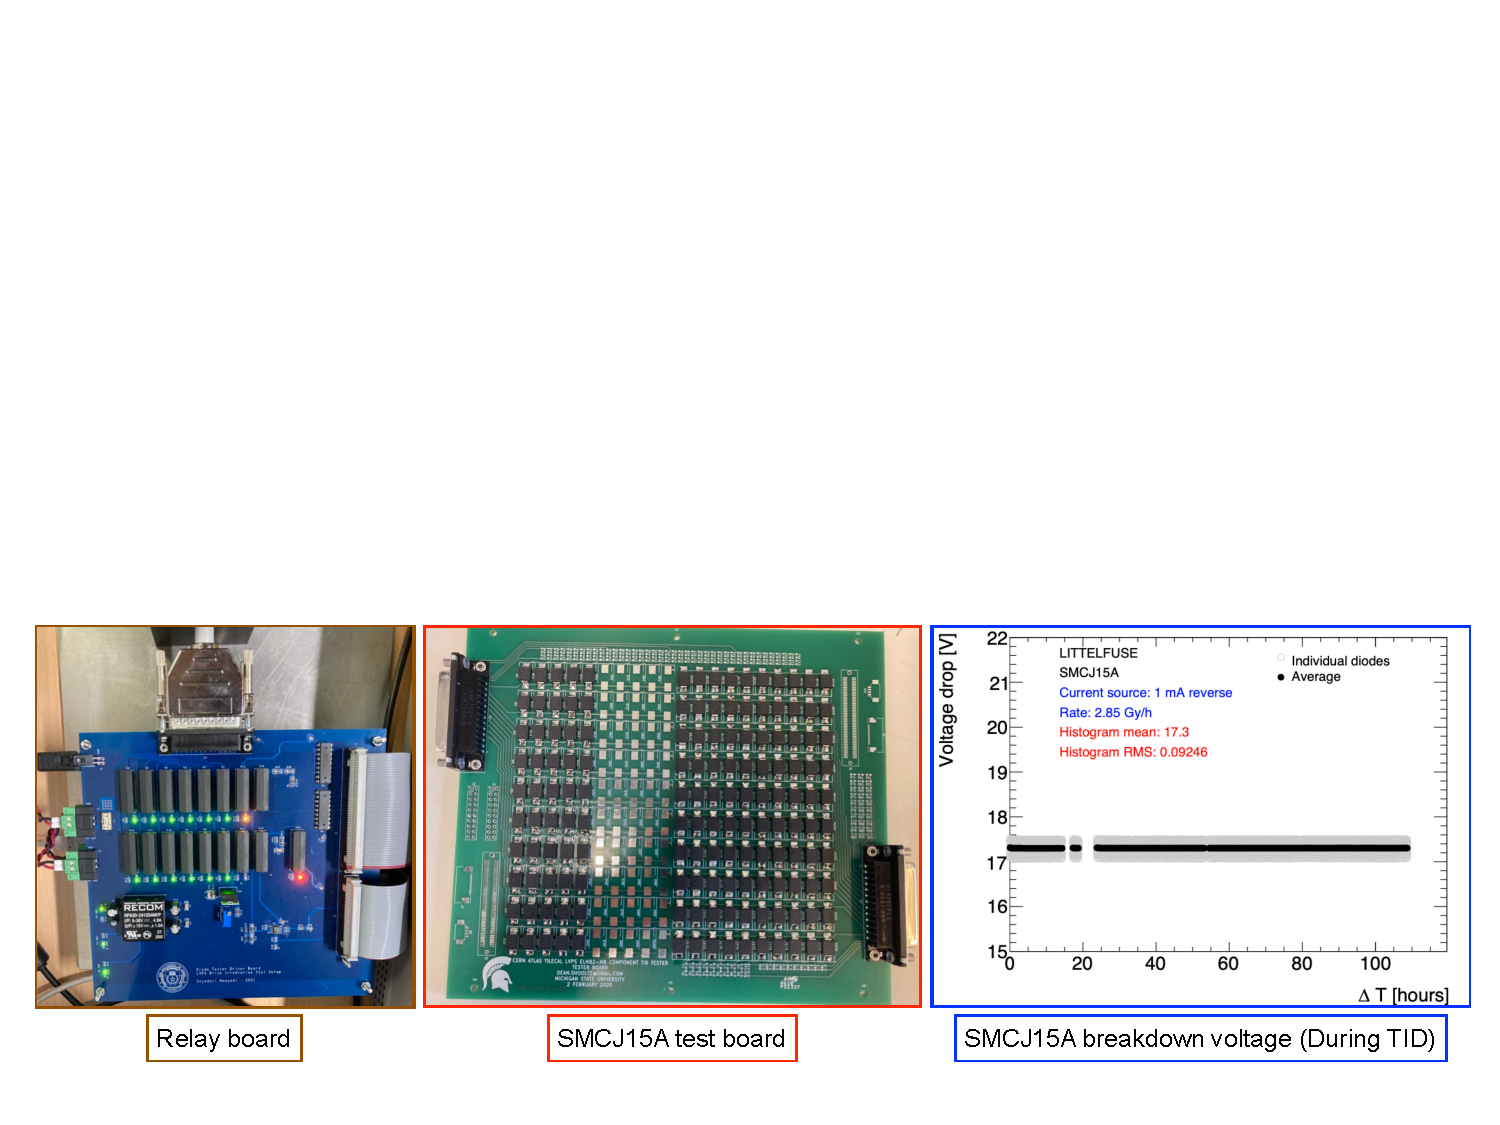
\includegraphics[width=1.0\linewidth]{assets/fig_diodes_tid_test.pdf}\\[2mm]
        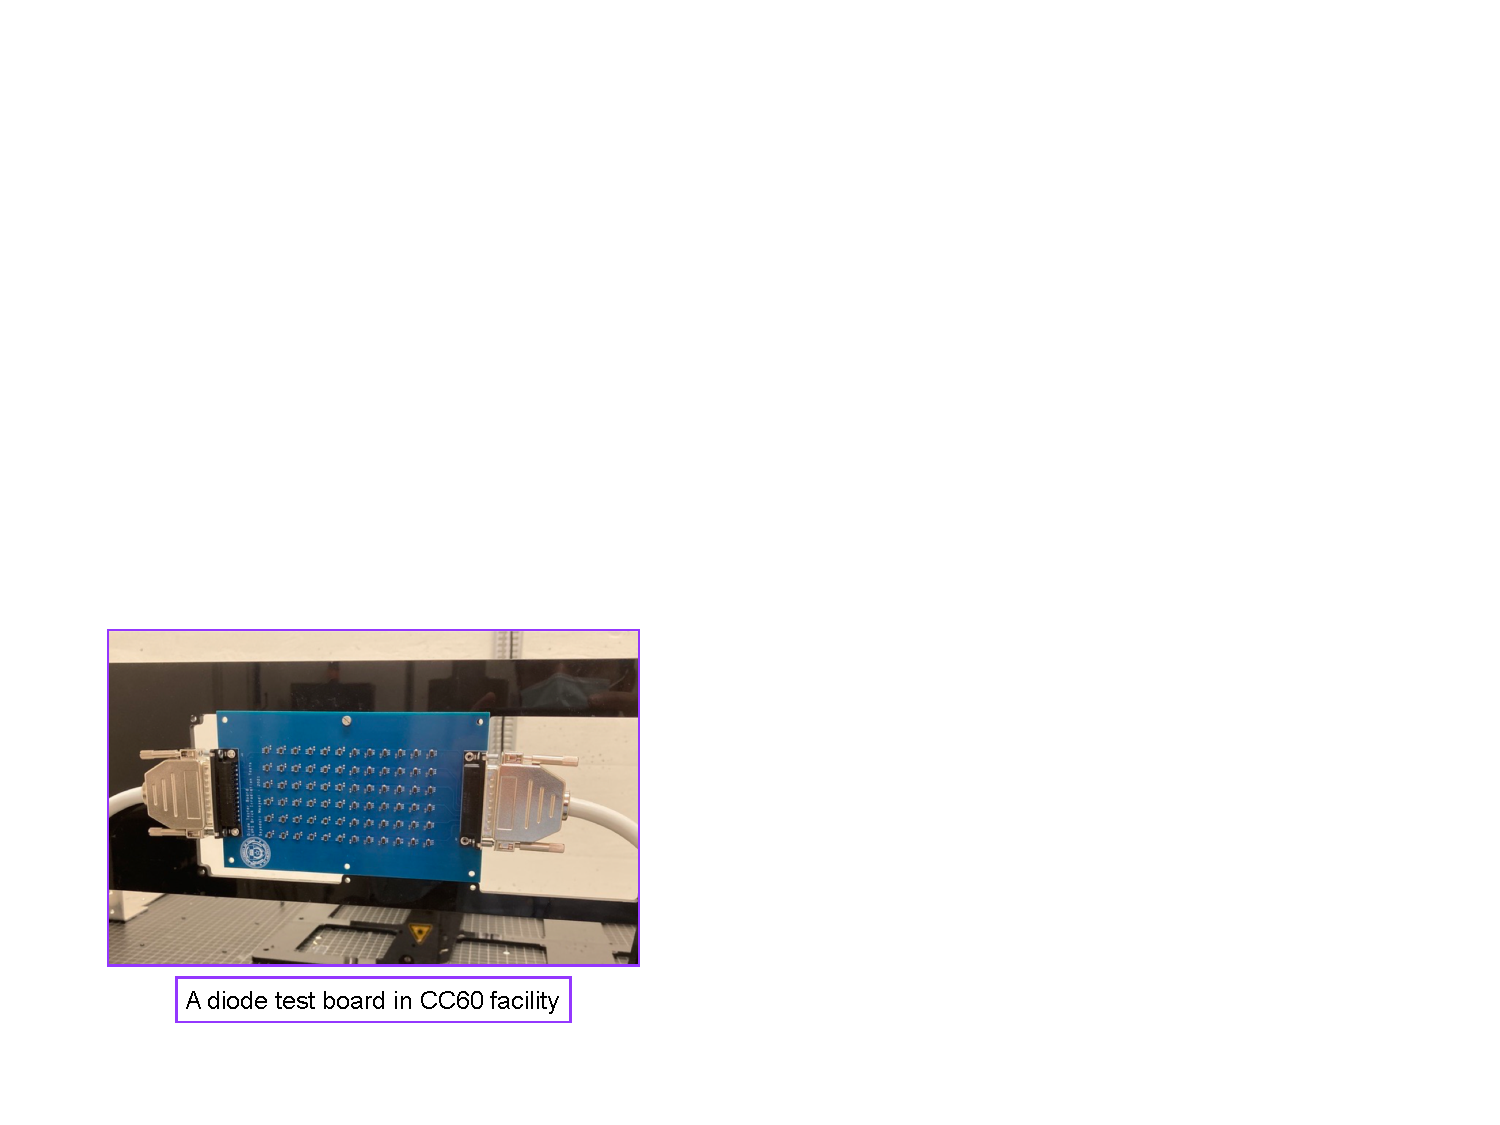
\includegraphics[width=1.0\linewidth]{assets/fig_diodes_niel_test.pdf}
    \end{center}
    \vspace{-0.3cm}
    \captiontext{Diode forward voltage stability under TID (top) and NIEL (bottom) irradiation.}
}

\block{Dosimetry Methodologies}{
    \looseitems
        \item Accurate dosimetry during component irradiation is as critical as the irradiation itself to prevent under-qualification.
        \item Standard alanine dosimeters were utilized to accurately measure the absorbed \textcolor{tid}{TID} during Gamma irradiation at CERN CC60.
        \item For \textcolor{niel}{NIEL} testing, activation foils provided a precise integration of the non-thermal neutron fluence at the TRIGA reactor.
        \item The meticulous dosimetric correlation ensures that all applied Safety Factors (SF) are grounded in absolute, traceable physical measurements.
    \end{itemize}
}

\block{References}{
    \small
    \begin{enumerate}\setlength{\itemsep}{0.1em}
        \item S. Moayedi (ATLAS), \emph{Upgrade of the ATLAS Tile Calorimeter
        Front-End Power Supply for the HL-LHC}, TWEPP 2025.
        \item ATLAS Collaboration, \emph{Technical Design Report for the Phase-II
        Upgrade of the ATLAS Tile Calorimeter}, CERN-LHCC-2017-019 (2018).
    \end{enumerate}
}

% ===========================================================================
%  COLUMN 2
% ===========================================================================
\column{0.333}

\block{Isolation Amplifiers: SI8920 vs HCPL7800}{
    \tightitems
        \item Galvanic isolation is a critical requirement in the sensing circuits to prevent ground loops and protect the sensitive low-voltage readout electronics from high-voltage surges. We systematically evaluated two primary candidates: the \textbf{SI8920} and the \textbf{HCPL7800}.
        \item The \textbf{SI8920} demonstrated extreme stability across the required operational bounds. When properly constrained to an input voltage $\leq 100\,\text{mV}$, it exhibited minimal gain degradation under \textcolor{tid}{TID} exposure, significantly outperforming the pre-defined safety requirements.
        \item In stark contrast, the \textbf{HCPL7800} exhibited a catastrophic gain collapse during \textcolor{niel}{NIEL} testing. 
        \item The internal optocoupling mechanism of the HCPL7800 suffered severe lattice displacement damage from neutron bombardment.
        \item It completely failed to transmit analog signals linearly at a fluence of $2.75\times10^{12}\,\text{n}_{\text{eq}}/\text{cm}^2$, forcing its immediate removal from the final design iteration.
    \end{itemize}
    \vspace{0.1cm}
    \begin{center}
        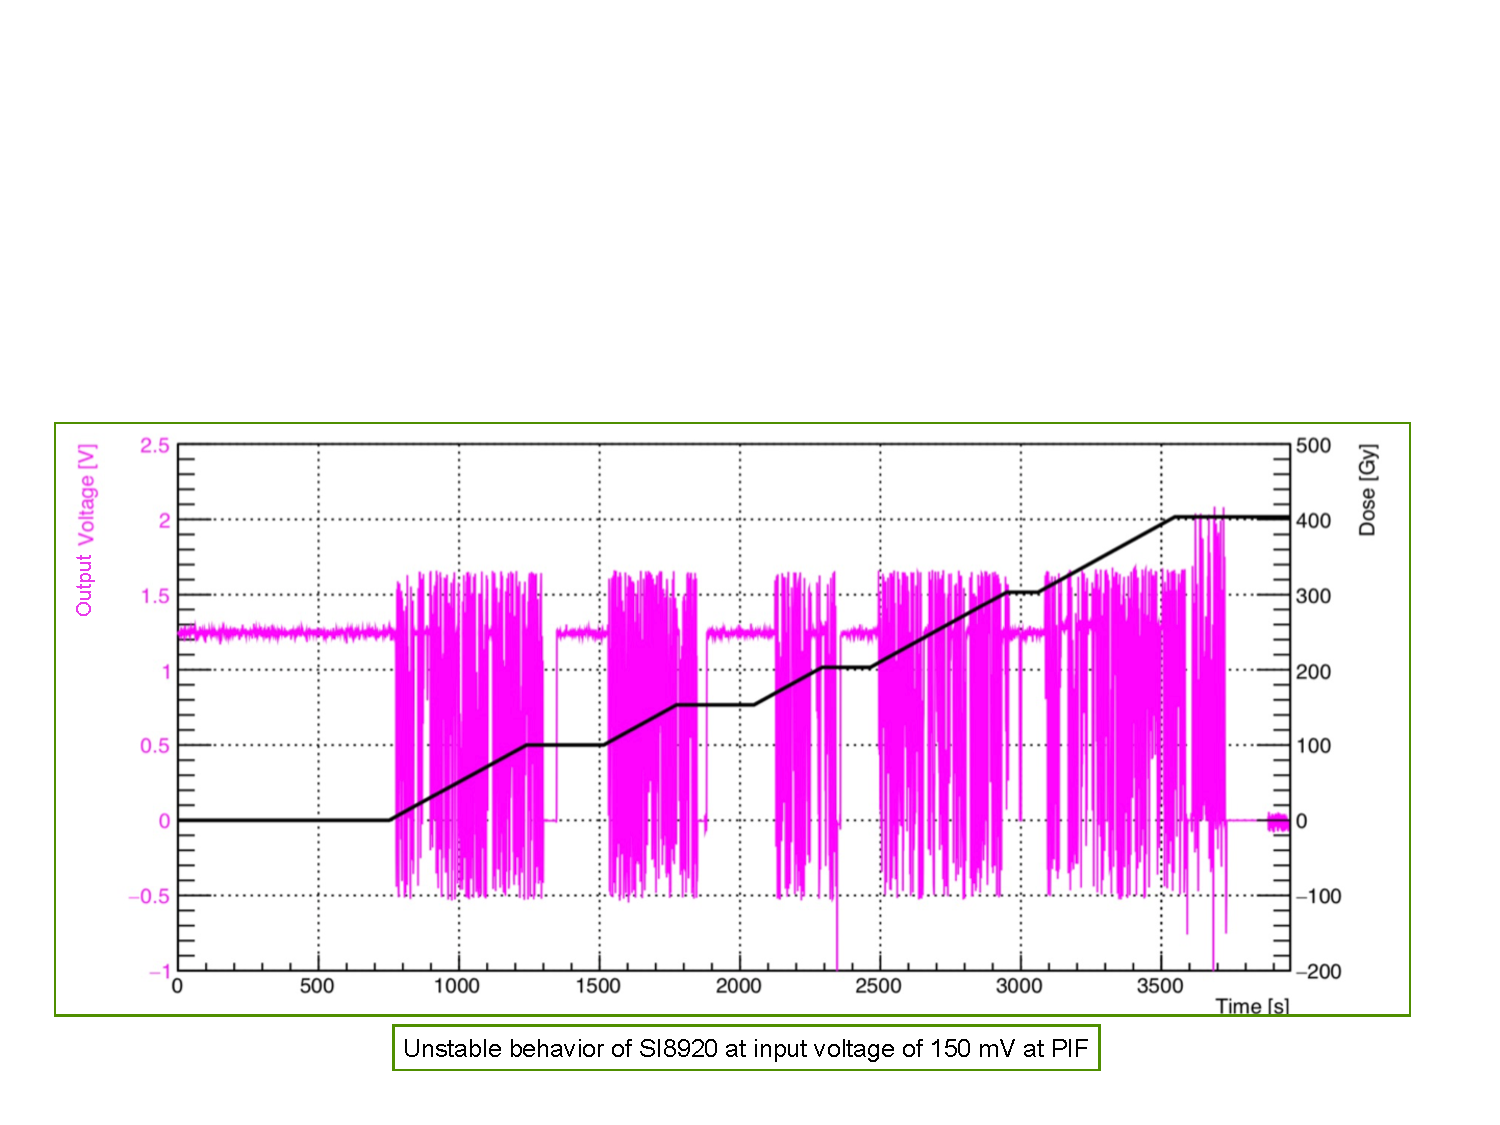
\includegraphics[width=1.0\linewidth]{assets/fig_si8920_isolation_amp.pdf}
    \end{center}
    \vspace{-0.3cm}
    \captiontext{SI8920 amplifier gain stability as a function of TID.}
}

\block{Signal Fidelity Under High Fluence}{
    \tightitems
        \item The catastrophic failure of the HCPL7800 underscores the absolute necessity of rigorous component-level testing; macroscopic system-level tests often mask specific vulnerabilities until an irreversible cascade failure occurs in the field.
        \item The degradation profile of the optocoupler was characterized by an exponentially decaying Current Transfer Ratio (CTR) as neutron fluence increased.
        \item Identifying this specific breakdown mode before finalizing the PCB layout prevented a critical systemic weakness in the High-Voltage distribution network.
        \item Subsequent thermal annealing phases demonstrated minimal recovery for the optocoupler, indicating permanent displacement damage.
    \end{itemize}
    \vspace{0.1cm}
    \begin{center}
        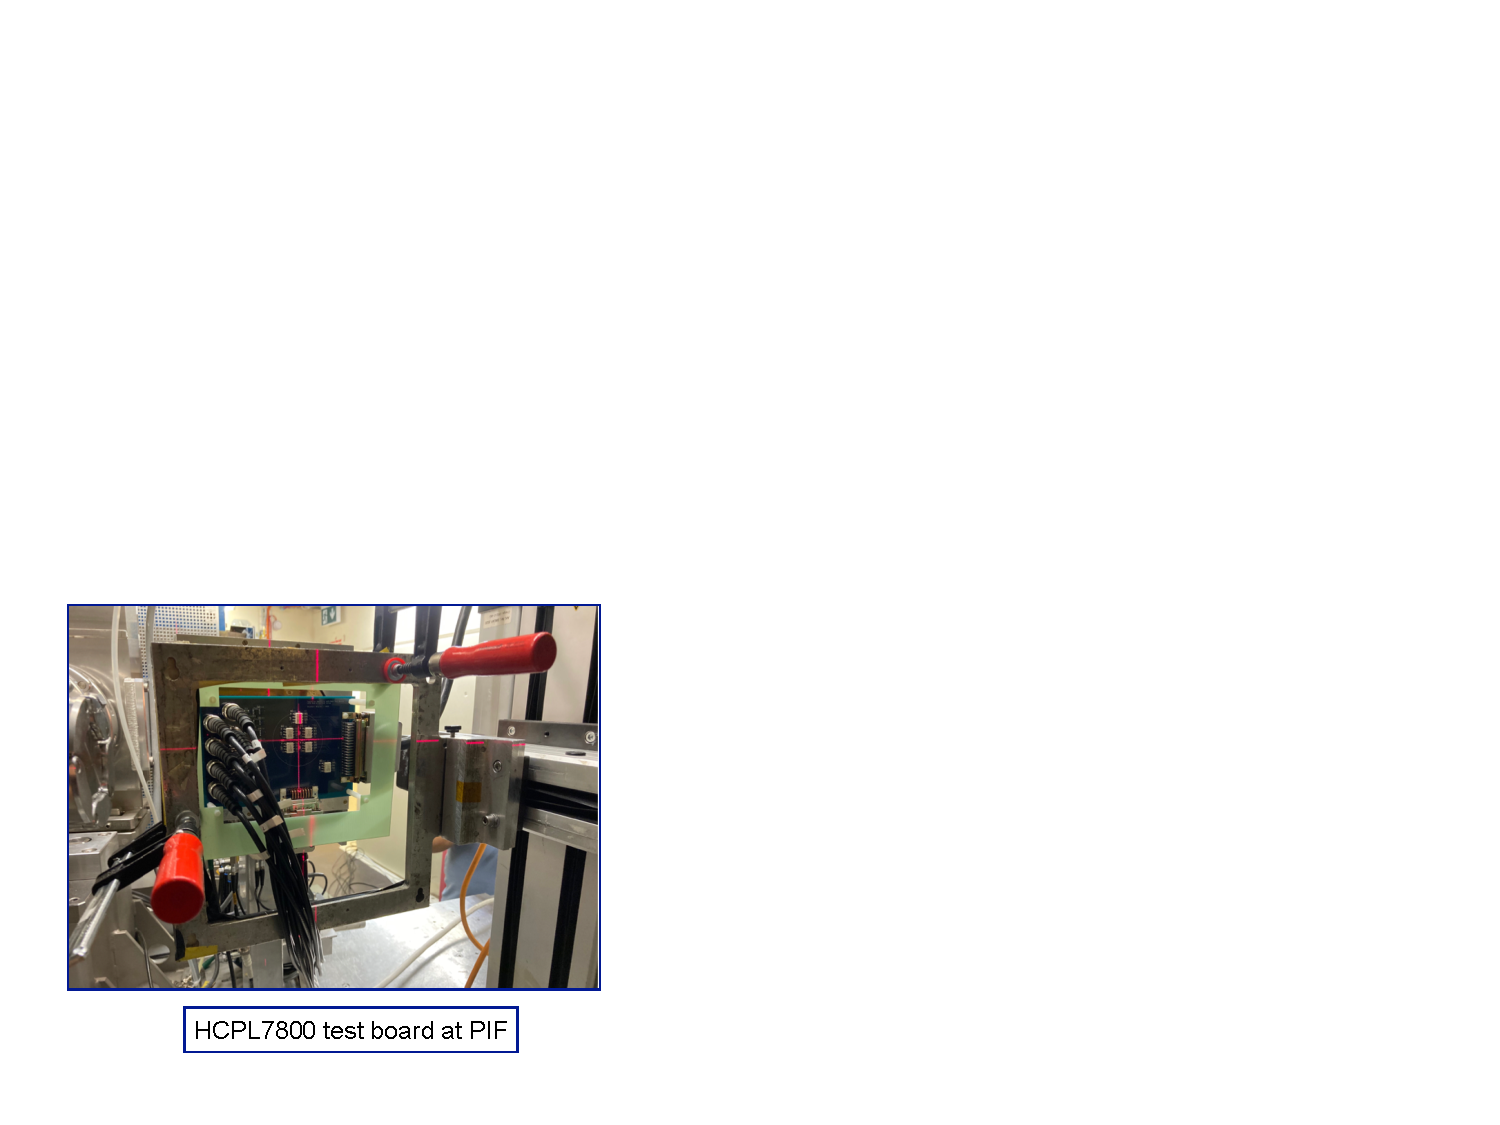
\includegraphics[width=1.0\linewidth]{assets/fig_hcpl7800_isolation_amp.pdf}
    \end{center}
    \vspace{-0.3cm}
    \captiontext{HCPL7800 catastrophic failure curve under escalating NIEL fluence.}
}

\block{Capacitor Degradation Analysis}{
    \tightitems
        \item High-value multi-layer ceramic capacitors (MLCCs) and specialized polymer electrolytic capacitors were tested for Equivalent Series Resistance (ESR) drift under extreme \textcolor{tid}{TID}.
        \item No significant capacitance loss or ESR escalation was recorded up to $100\,\text{Gy}$, guaranteeing stable filtering of the $300\,\text{kHz}$ ripple in the LVPS architecture.
        \item Polymer variants demonstrated a slight advantage in transient recovery over older tantalum counterparts.
    \end{itemize}
    \vspace{0.2cm}
    \begin{center}
    \small
    \resizebox{\linewidth}{!}{
    \begin{tabular}{|p{0.45\linewidth}|p{0.55\linewidth}|}
    \hline
    \textbf{Capacitor Type} & \textbf{Post-Irradiation Behavior} \\
    \hline
    \textbf{MLCC (X7R)} & Capacitance stable within $\pm 5\%$ \\
    \hline
    \textbf{Polymer Aluminum} & ESR drift $< 2\,\text{m}\Omega$ \\
    \hline
    \textbf{Tantalum (Legacy)} & Higher ESR drift, deprecated \\
    \hline
    \end{tabular}
    }
    \end{center}
    \vspace{0.1cm}
}

\block{Passive Component Survival Margins}{
    \tightitems
        \item Standard thick-film and thin-film resistors experienced virtually zero measurable shift in resistance, maintaining tight $0.1\%$ tolerances necessary for precision ADCs.
        \item Ferrite cores utilized in the custom LVPS transformers were tested for magnetic permeability reduction, with results confirming minimal impact on the BH-curve saturation characteristics.
        \item This empirical evidence solidifies the long-term passive filtering capability of the overall architecture.
    \end{itemize}
}

% ===========================================================================
%  COLUMN 3
% ===========================================================================
\column{0.333}

\block{Power Control Components}{
    \looseitems
        \item The LVPS brick architecture utilizes the \textbf{IR2110 MOSFET driver} to control the primary high-frequency switching stage of the forward converter.
        \item Maintaining precise timing is critical; any drift in propagation delay could lead to simultaneous conduction (shoot-through) of the primary MOSFETs, instantly destroying the brick.
        \item Irradiation testing rigorously verified that the driver maintains sufficiently fast rise and fall times, and that propagation delays do not drift into dangerous regions, even at peak HL-LHC expected doses.
        \item The IR2110's internal level-shifting circuitry proved exceptionally resilient to both ionizing and non-ionizing damage.
    \end{itemize}
    \vspace{0.1cm}
    \begin{center}
        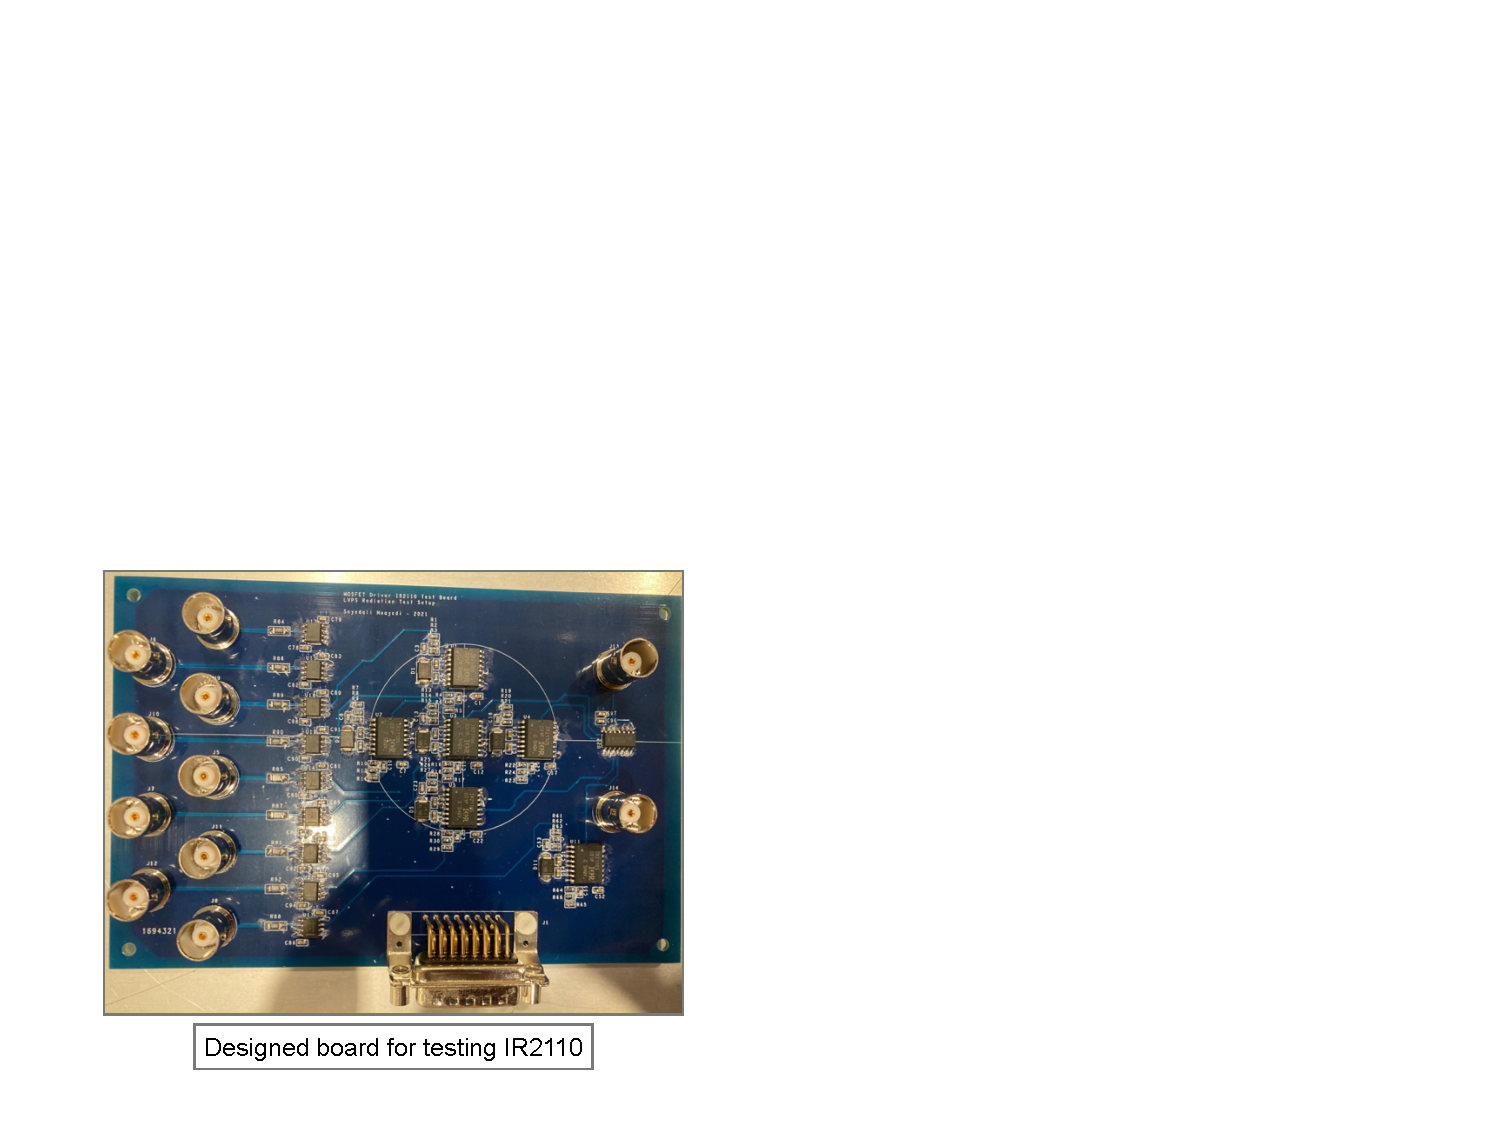
\includegraphics[width=1.0\linewidth]{assets/fig_ir2110_mosfet_driver.pdf}
    \end{center}
    \vspace{-0.3cm}
    \captiontext{IR2110 MOSFET driver propagation delay stability during irradiation.}
}

\block{High-Voltage Switching MOSFETs}{
    \looseitems
        \item The main switching element, the \textbf{SIHFS9N60A MOSFET}, was heavily scrutinized for drain-source breakdown degradation and threshold voltage shifts.
        \item A positive shift in threshold voltage indicates charge trapping in the gate oxide, a primary failure mode under \textcolor{tid}{TID}.
        \item Under continuous irradiation, the pre-production MOSFETs maintained operational integrity up to $323\,\text{Gy}$, surviving well beyond the stringent $80\,\text{Gy}$ specification baseline.
        \item This massive safety margin provides absolute confidence in the longevity of the LVPS bricks over the planned 10-year operational span.
    \end{itemize}
    \vspace{0.1cm}
    \begin{center}
        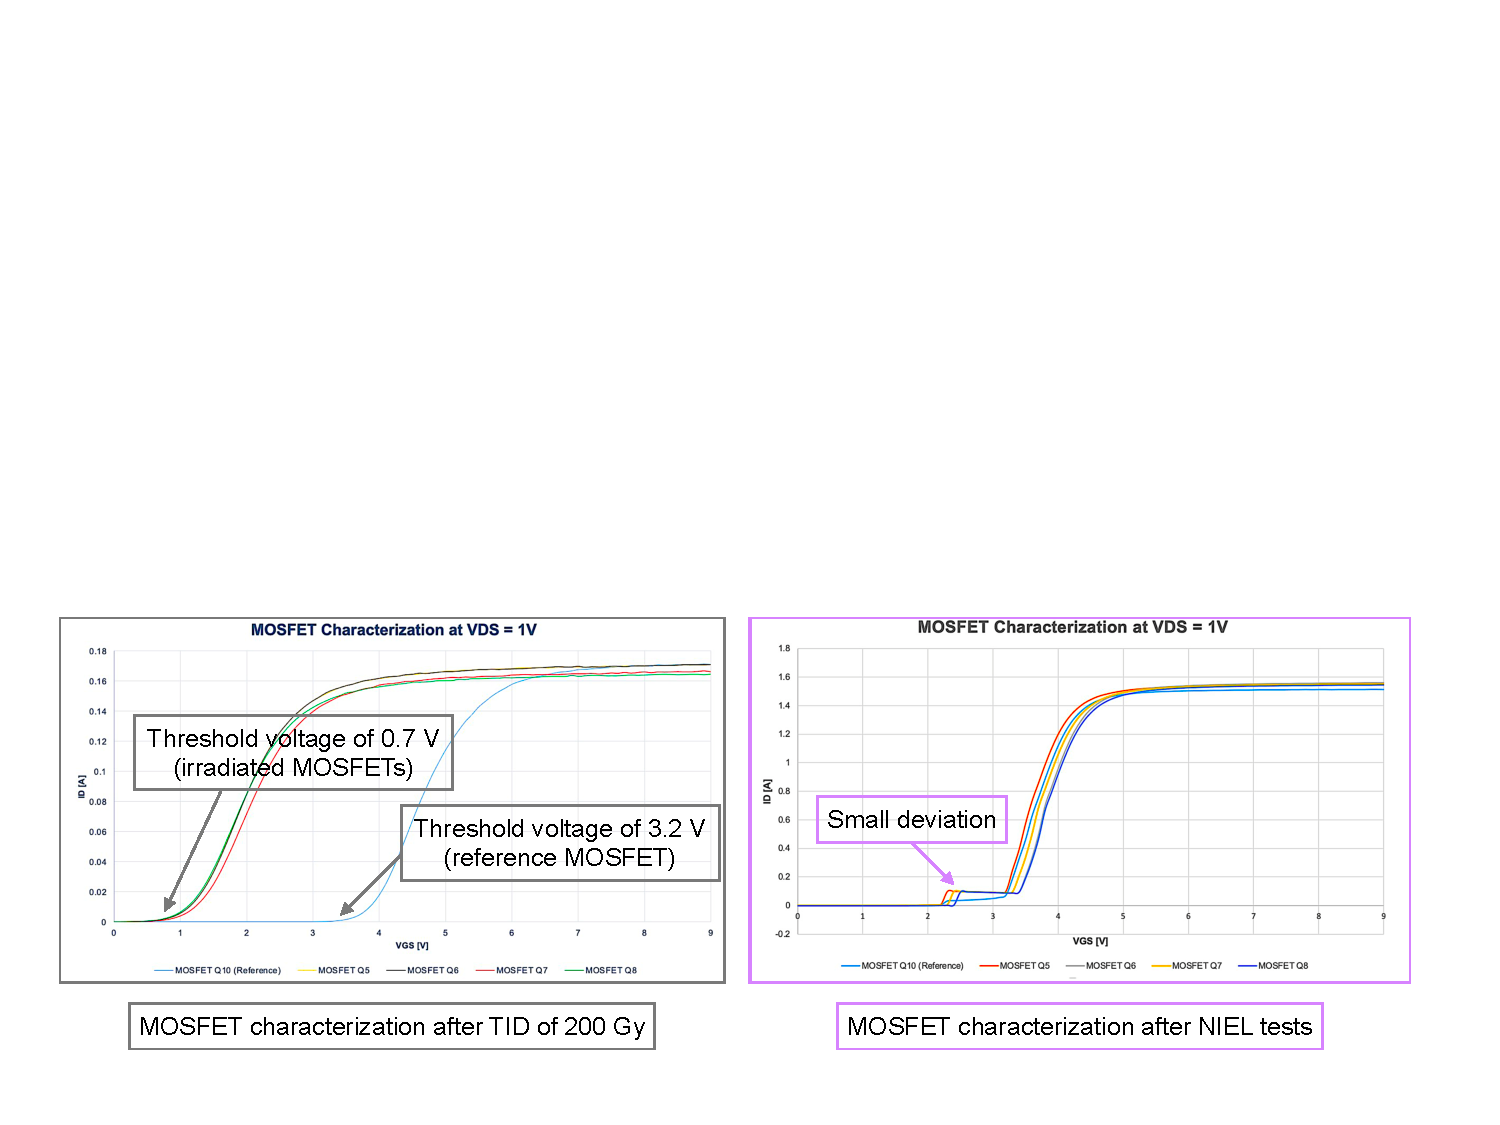
\includegraphics[width=1.0\linewidth]{assets/fig_sihfs9n60a_mosfet.pdf}
    \end{center}
    \vspace{-0.3cm}
    \captiontext{SIHFS9N60A MOSFET threshold voltage variation vs TID.}
}

\block{Voltage Regulators and References}{
    \looseitems
        \item Commercial voltage regulators (such as the \textbf{LT3080}) are responsible for generating localized low-noise logic-level rails.
        \item During \textcolor{tid}{TID} sweeps, the LT3080 exhibited a maximum output drift of $<1.5\%$, well within the $5\%$ operational tolerance required by the digital ASICs.
        \item Precision voltage references essential for the ADCs maintained accuracy within parts-per-million (ppm) tolerances despite prolonged neutron displacement exposure.
    \end{itemize}
}

\block{Data Aggregation Architecture}{
    \looseitems
        \item All successfully verified component models are permanently entered into the global ATLAS component database.
        \item The stringent lot-tracking system implemented guarantees that no untested or unverified silicon wafer batches can accidentally be integrated during the mass assembly phases.
        \item Any future revisions must undergo the exact same tri-fold irradiation sequence before approval.
    \end{itemize}
}

\block{Conclusions}{
    \looseitems
        \item The component-level testing campaign successfully isolated highly vulnerable commercial elements (e.g., the HCPL7800 optocoupler) and confirmed the extreme resilience of selected alternatives (e.g., SI8920, SIHFS9N60A).
        \item Every semiconductor selected for the Phase-II electronics production run has been empirically validated to withstand the HL-LHC environment with substantial safety margins.
        \item This rigorous methodology ensures that the fully assembled ATLAS TileCal Minidrawers will not succumb to premature component failures due to radiation damage.
    \end{itemize}
}

\end{columns}
\end{document}
